\subsubsection{17.11.2015}
\textit{\textbf{Time frame:}} 17:00-21:30 \newline
The module for scoring climbers was assembled and tested.

\begin{figure}[H]
	\begin{minipage}[h]{1\linewidth}
		\center{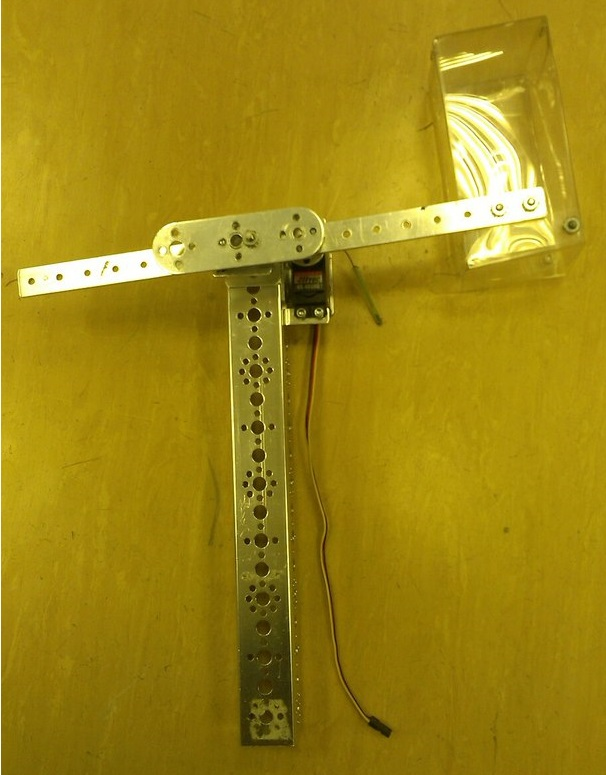
\includegraphics[scale=0.2]{3Engineering/5Team_meetings/days_of_meetings/17.11.2015/images/01}}
		\caption{module for scoring climbers}
	\end{minipage}
\end{figure}

Mechanism for opening the cover worked stable.The principle of work of the current mechanism is following: the pin, that fastens cover to the bucket is tied to the mount of the axis by thread. When the container overturns, the thread stretches and pulls the pin.

\begin{figure}[H]
	\begin{minipage}[h]{0.31\linewidth}
		\center{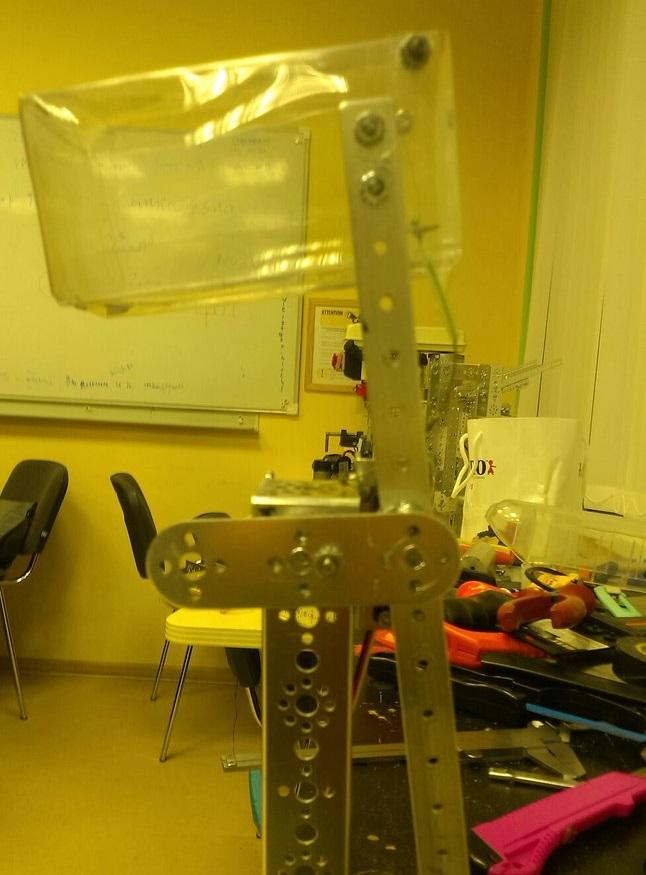
\includegraphics[scale=0.18]{3Engineering/5Team_meetings/days_of_meetings/17.11.2015/images/02}}
	\end{minipage}
	\begin{minipage}[h]{0.31\linewidth}
		\center{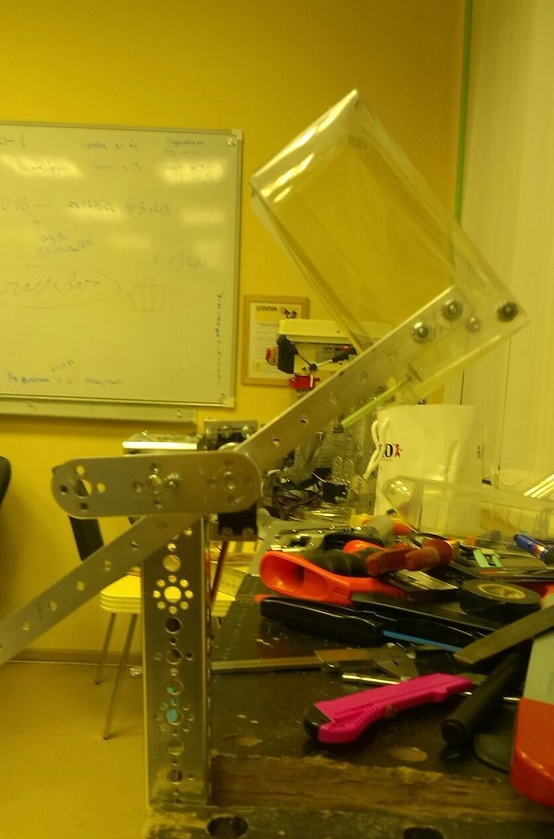
\includegraphics[scale=0.19]{3Engineering/5Team_meetings/days_of_meetings/17.11.2015/images/03}}
	\end{minipage}
	\begin{minipage}[h]{0.31\linewidth}
		\center{
\includegraphics[scale=0.23]{3Engineering/5Team_meetings/days_of_meetings/17.11.2015/images/04}}
	\end{minipage}
	\caption{the principle of work}
\end{figure}


